% Options for packages loaded elsewhere
\PassOptionsToPackage{unicode}{hyperref}
\PassOptionsToPackage{hyphens}{url}
\PassOptionsToPackage{dvipsnames,svgnames,x11names}{xcolor}
%
\documentclass[
]{article}

\usepackage{amsmath,amssymb}
\usepackage{iftex}
\ifPDFTeX
  \usepackage[T1]{fontenc}
  \usepackage[utf8]{inputenc}
  \usepackage{textcomp} % provide euro and other symbols
\else % if luatex or xetex
  \usepackage{unicode-math}
  \defaultfontfeatures{Scale=MatchLowercase}
  \defaultfontfeatures[\rmfamily]{Ligatures=TeX,Scale=1}
\fi
\usepackage{lmodern}
\ifPDFTeX\else  
    % xetex/luatex font selection
\fi
% Use upquote if available, for straight quotes in verbatim environments
\IfFileExists{upquote.sty}{\usepackage{upquote}}{}
\IfFileExists{microtype.sty}{% use microtype if available
  \usepackage[]{microtype}
  \UseMicrotypeSet[protrusion]{basicmath} % disable protrusion for tt fonts
}{}
\makeatletter
\@ifundefined{KOMAClassName}{% if non-KOMA class
  \IfFileExists{parskip.sty}{%
    \usepackage{parskip}
  }{% else
    \setlength{\parindent}{0pt}
    \setlength{\parskip}{6pt plus 2pt minus 1pt}}
}{% if KOMA class
  \KOMAoptions{parskip=half}}
\makeatother
\usepackage{xcolor}
\usepackage[lmargin=20mm,rmargin=20mm]{geometry}
\setlength{\emergencystretch}{3em} % prevent overfull lines
\setcounter{secnumdepth}{5}
% Make \paragraph and \subparagraph free-standing
\makeatletter
\ifx\paragraph\undefined\else
  \let\oldparagraph\paragraph
  \renewcommand{\paragraph}{
    \@ifstar
      \xxxParagraphStar
      \xxxParagraphNoStar
  }
  \newcommand{\xxxParagraphStar}[1]{\oldparagraph*{#1}\mbox{}}
  \newcommand{\xxxParagraphNoStar}[1]{\oldparagraph{#1}\mbox{}}
\fi
\ifx\subparagraph\undefined\else
  \let\oldsubparagraph\subparagraph
  \renewcommand{\subparagraph}{
    \@ifstar
      \xxxSubParagraphStar
      \xxxSubParagraphNoStar
  }
  \newcommand{\xxxSubParagraphStar}[1]{\oldsubparagraph*{#1}\mbox{}}
  \newcommand{\xxxSubParagraphNoStar}[1]{\oldsubparagraph{#1}\mbox{}}
\fi
\makeatother


\providecommand{\tightlist}{%
  \setlength{\itemsep}{0pt}\setlength{\parskip}{0pt}}\usepackage{longtable,booktabs,array}
\usepackage{calc} % for calculating minipage widths
% Correct order of tables after \paragraph or \subparagraph
\usepackage{etoolbox}
\makeatletter
\patchcmd\longtable{\par}{\if@noskipsec\mbox{}\fi\par}{}{}
\makeatother
% Allow footnotes in longtable head/foot
\IfFileExists{footnotehyper.sty}{\usepackage{footnotehyper}}{\usepackage{footnote}}
\makesavenoteenv{longtable}
\usepackage{graphicx}
\makeatletter
\def\maxwidth{\ifdim\Gin@nat@width>\linewidth\linewidth\else\Gin@nat@width\fi}
\def\maxheight{\ifdim\Gin@nat@height>\textheight\textheight\else\Gin@nat@height\fi}
\makeatother
% Scale images if necessary, so that they will not overflow the page
% margins by default, and it is still possible to overwrite the defaults
% using explicit options in \includegraphics[width, height, ...]{}
\setkeys{Gin}{width=\maxwidth,height=\maxheight,keepaspectratio}
% Set default figure placement to htbp
\makeatletter
\def\fps@figure{htbp}
\makeatother

\usepackage{booktabs}
\usepackage{longtable}
\usepackage{array}
\usepackage{multirow}
\usepackage{wrapfig}
\usepackage{float}
\usepackage{colortbl}
\usepackage{pdflscape}
\usepackage{tabu}
\usepackage{threeparttable}
\usepackage{threeparttablex}
\usepackage[normalem]{ulem}
\usepackage{makecell}
\usepackage{xcolor}
\usepackage{lineno}\linenumbers
\usepackage{pdflscape}
\usepackage[inkscapeformat=png]{svg}
\usepackage{kbordermatrix}
\usepackage{wrapfig}
\usepackage{amsmath}
\DeclareMathOperator*{\argmin}{arg\,min}
\makeatletter
\@ifpackageloaded{caption}{}{\usepackage{caption}}
\AtBeginDocument{%
\ifdefined\contentsname
  \renewcommand*\contentsname{Table of contents}
\else
  \newcommand\contentsname{Table of contents}
\fi
\ifdefined\listfigurename
  \renewcommand*\listfigurename{List of Figures}
\else
  \newcommand\listfigurename{List of Figures}
\fi
\ifdefined\listtablename
  \renewcommand*\listtablename{List of Tables}
\else
  \newcommand\listtablename{List of Tables}
\fi
\ifdefined\figurename
  \renewcommand*\figurename{Supplemantary

Figure}
\else
  \newcommand\figurename{Supplemantary

Figure}
\fi
\ifdefined\tablename
  \renewcommand*\tablename{Table}
\else
  \newcommand\tablename{Table}
\fi
}
\@ifpackageloaded{float}{}{\usepackage{float}}
\floatstyle{ruled}
\@ifundefined{c@chapter}{\newfloat{codelisting}{h}{lop}}{\newfloat{codelisting}{h}{lop}[chapter]}
\floatname{codelisting}{Listing}
\newcommand*\listoflistings{\listof{codelisting}{List of Listings}}
\makeatother
\makeatletter
\makeatother
\makeatletter
\@ifpackageloaded{caption}{}{\usepackage{caption}}
\@ifpackageloaded{subcaption}{}{\usepackage{subcaption}}
\makeatother

\ifLuaTeX
  \usepackage{selnolig}  % disable illegal ligatures
\fi
\usepackage[style=authoryear,]{biblatex}
\addbibresource{library.bib}
\usepackage{bookmark}

\IfFileExists{xurl.sty}{\usepackage{xurl}}{} % add URL line breaks if available
\urlstyle{same} % disable monospaced font for URLs
\hypersetup{
  pdftitle={Supplementary Material},
  pdfauthor={James Adams, Michiel de Vries, Chaozhi Zheng, \& Fred van Eeuwijk},
  colorlinks=true,
  linkcolor={blue},
  filecolor={Maroon},
  citecolor={Blue},
  urlcolor={Blue},
  pdfcreator={LaTeX via pandoc}}




\section{Founder Origin Sparsity}\label{founder-origin-sparsity}

After the conclusion of the RABBIT pipeline, founder origin sparsity was
assessed genome-wide using a rolling-window over average number of sites
which had no confident haplotype call (probability under 0.5). This
showed a high degree of missing haplotype calls on chromosome's 1 and 5
(Sup Fig~\ref{fig-sparse}).

\begin{figure}[h!]

\centering{

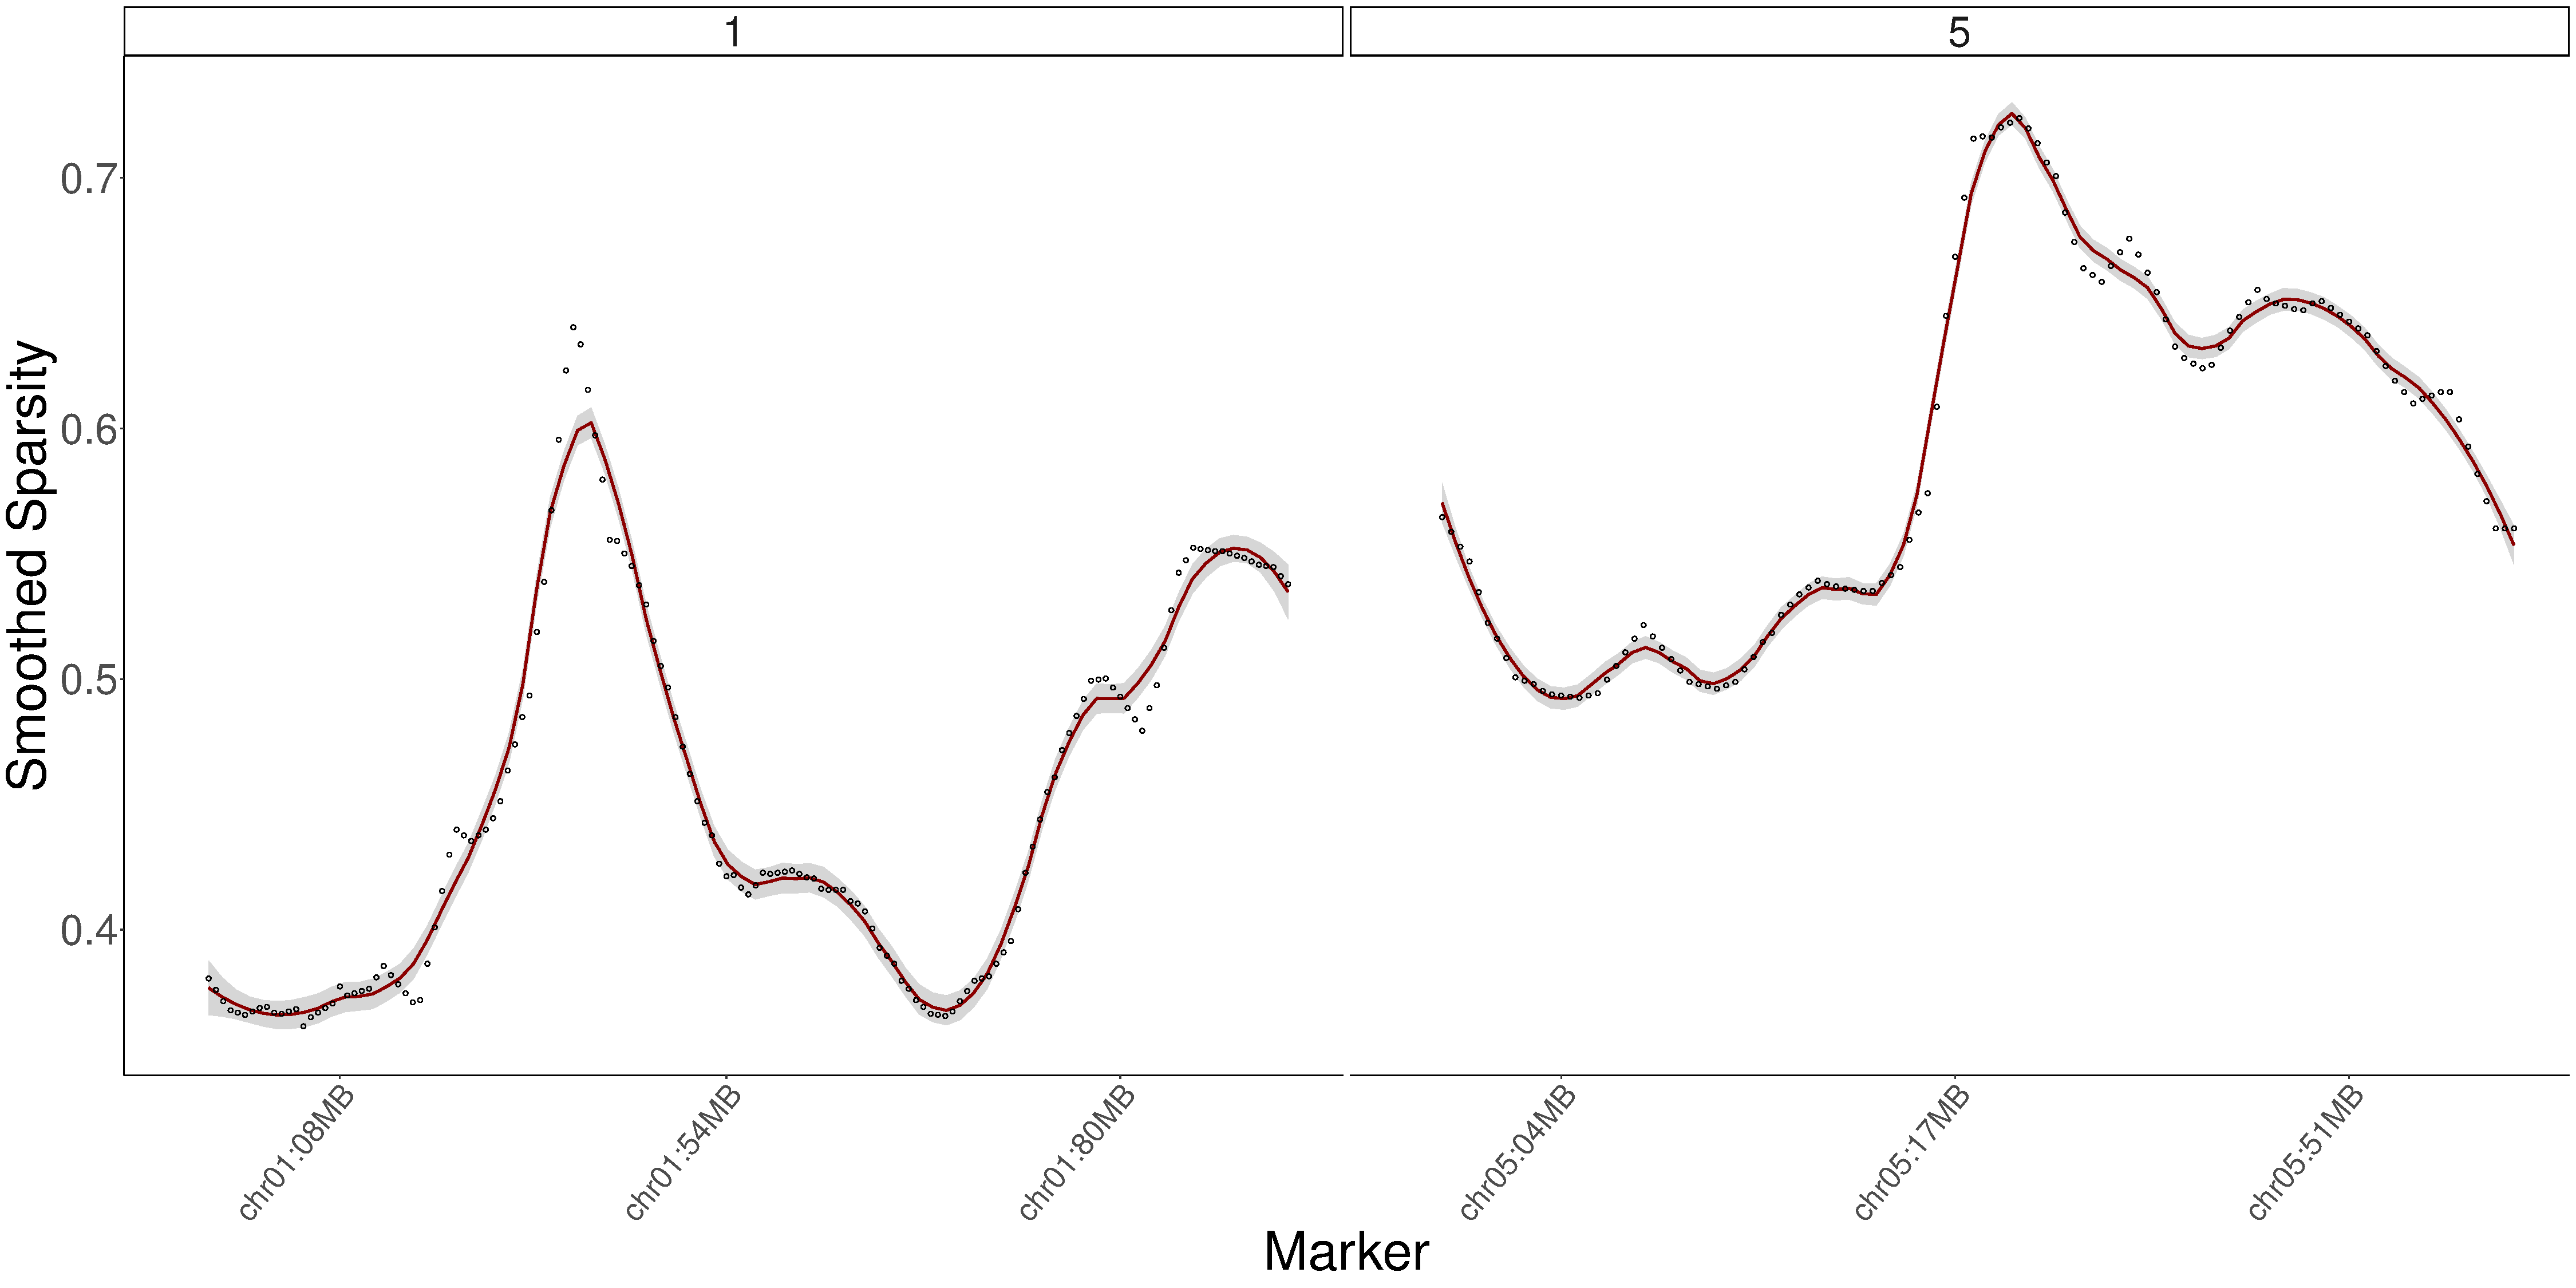
\includegraphics{supplementary_files/figure-pdf/fig-sparse-1.pdf}

}

\caption{\label{fig-sparse}Smoothed sparsity of founder-origin alleles
for chromosome's 1 and 5.}

\end{figure}%

\section{Multiallelic Marker Matrix
Parameterization}\label{multiallelic-marker-matrix-parameterization}

For both haplotag and IBD based markersets, let us assign each allele
some identifier \{a, b, c\} to denote genotypic states with the former
representing a haplotype sequence of 75 basepairs in length and the
latter being an assigned founder origin. We then consider two loci (l1
and l2) with the reference allele (\(a\)) being either the reference
haplotag allele or the most prevalent founder allele in the population.
The multiallelic incidence matrix is centred using the cross product of
a column vector of 1's
\(\left ( \mathbf{1}^T_4 = \left ( 1, 1, 1, 1 \right )^T \right )\) and
a vector of allelic frequencies excluding the reference allele
\(\left ( \mathbf{p} = \begin{bmatrix} l1b & l1c & l2b \\ \frac{3}{8} & \frac{1}{4} & \frac{1}{2}\end{bmatrix} \right )\).

\[
\begin{aligned}
\kbordermatrix{
    & l1 & l2 \\
  g1 & aa & ab  \\
  g2 & cc & bb  \\
  g3 & bb & aa  \\
  g4 & ab & ab   
} 
\Rightarrow
\kbordermatrix{
    & l1a & l1b & l1c & l2a & l2b \\
  g1 & 2 & 0 & 0 & 1 & 1 \\
  g2 & 0 & 0 & 2 & 0 & 2 \\
  g3 & 0 & 2 & 0 & 2 & 0 \\
  g4 & 1 & 1 & 0 & 1 & 1
}
\Rightarrow
\kbordermatrix{
    & l1b & l1c & l2b \\
  g1 & 0 & 0  & 1 \\
  g2 & 0 & 2  & 2 \\
  g3 & 2 & 0  & 0 \\
  g4 & 1 & 0  & 1 
}
\Rightarrow 
\\
\mathbf{1}^T_4 \bigotimes 2\mathbf{p} - \kbordermatrix{
    & l1b & l1c & l2b \\
  g1 & 0 & 0  & 1 \\
  g2 & 0 & 2  & 2 \\
  g3 & 2 & 0  & 0 \\
  g4 & 1 & 0  & 1 
}
\Rightarrow
\kbordermatrix{
    & l1b & l1c & l2b \\
  g1 & 2p_{l1b} & 2p_{l1c} & 2p_{l2b} - 1 \\
  g2 & 2p_{l1b} & 2p_{l1c} - 2  & 2p_{l2b} - 2 \\
  g3 & 2p_{l1b} - 2 & 2p_{l1c} & 2p_{l2b} \\
  g4 & 2p_{l1b} - 1 & 2p_{l1c}  & 2p_{l2b} - 1 
}
\Rightarrow
\kbordermatrix{
    & l1b & l1c & l2b \\
  g1 & \frac{3}{4} & \frac{1}{2} &  0 \\
  g2 & \frac{3}{4} & -\frac{3}{2}  & -1 \\
  g3 & -\frac{5}{4} & \frac{1}{2}  & 1 \\
  g4 & -\frac{1}{4}  & \frac{1}{2}  & 0 
}
\end{aligned}
\]

This centred matrix of either IBD founder or haplotag alleles was then
used in subsequent genome-wide regression models.


\section{LASSO and GROUP LASSO}\label{lasso-and-group-lasso}

For the LASSO (LS) training runs, the degrees of freedom and estimated
\(\lambda\) parameter were recorded. This is shown for all traits in
(Sup Fig~\ref{fig-lasso}). For the grouped LASSO (GLS), the predictive
accuracy of that training run is also captured and shown only for the
IBD probeset in (Sup Fig~\ref{fig-lasso-2}).

\begin{figure}[h!]

\centering{

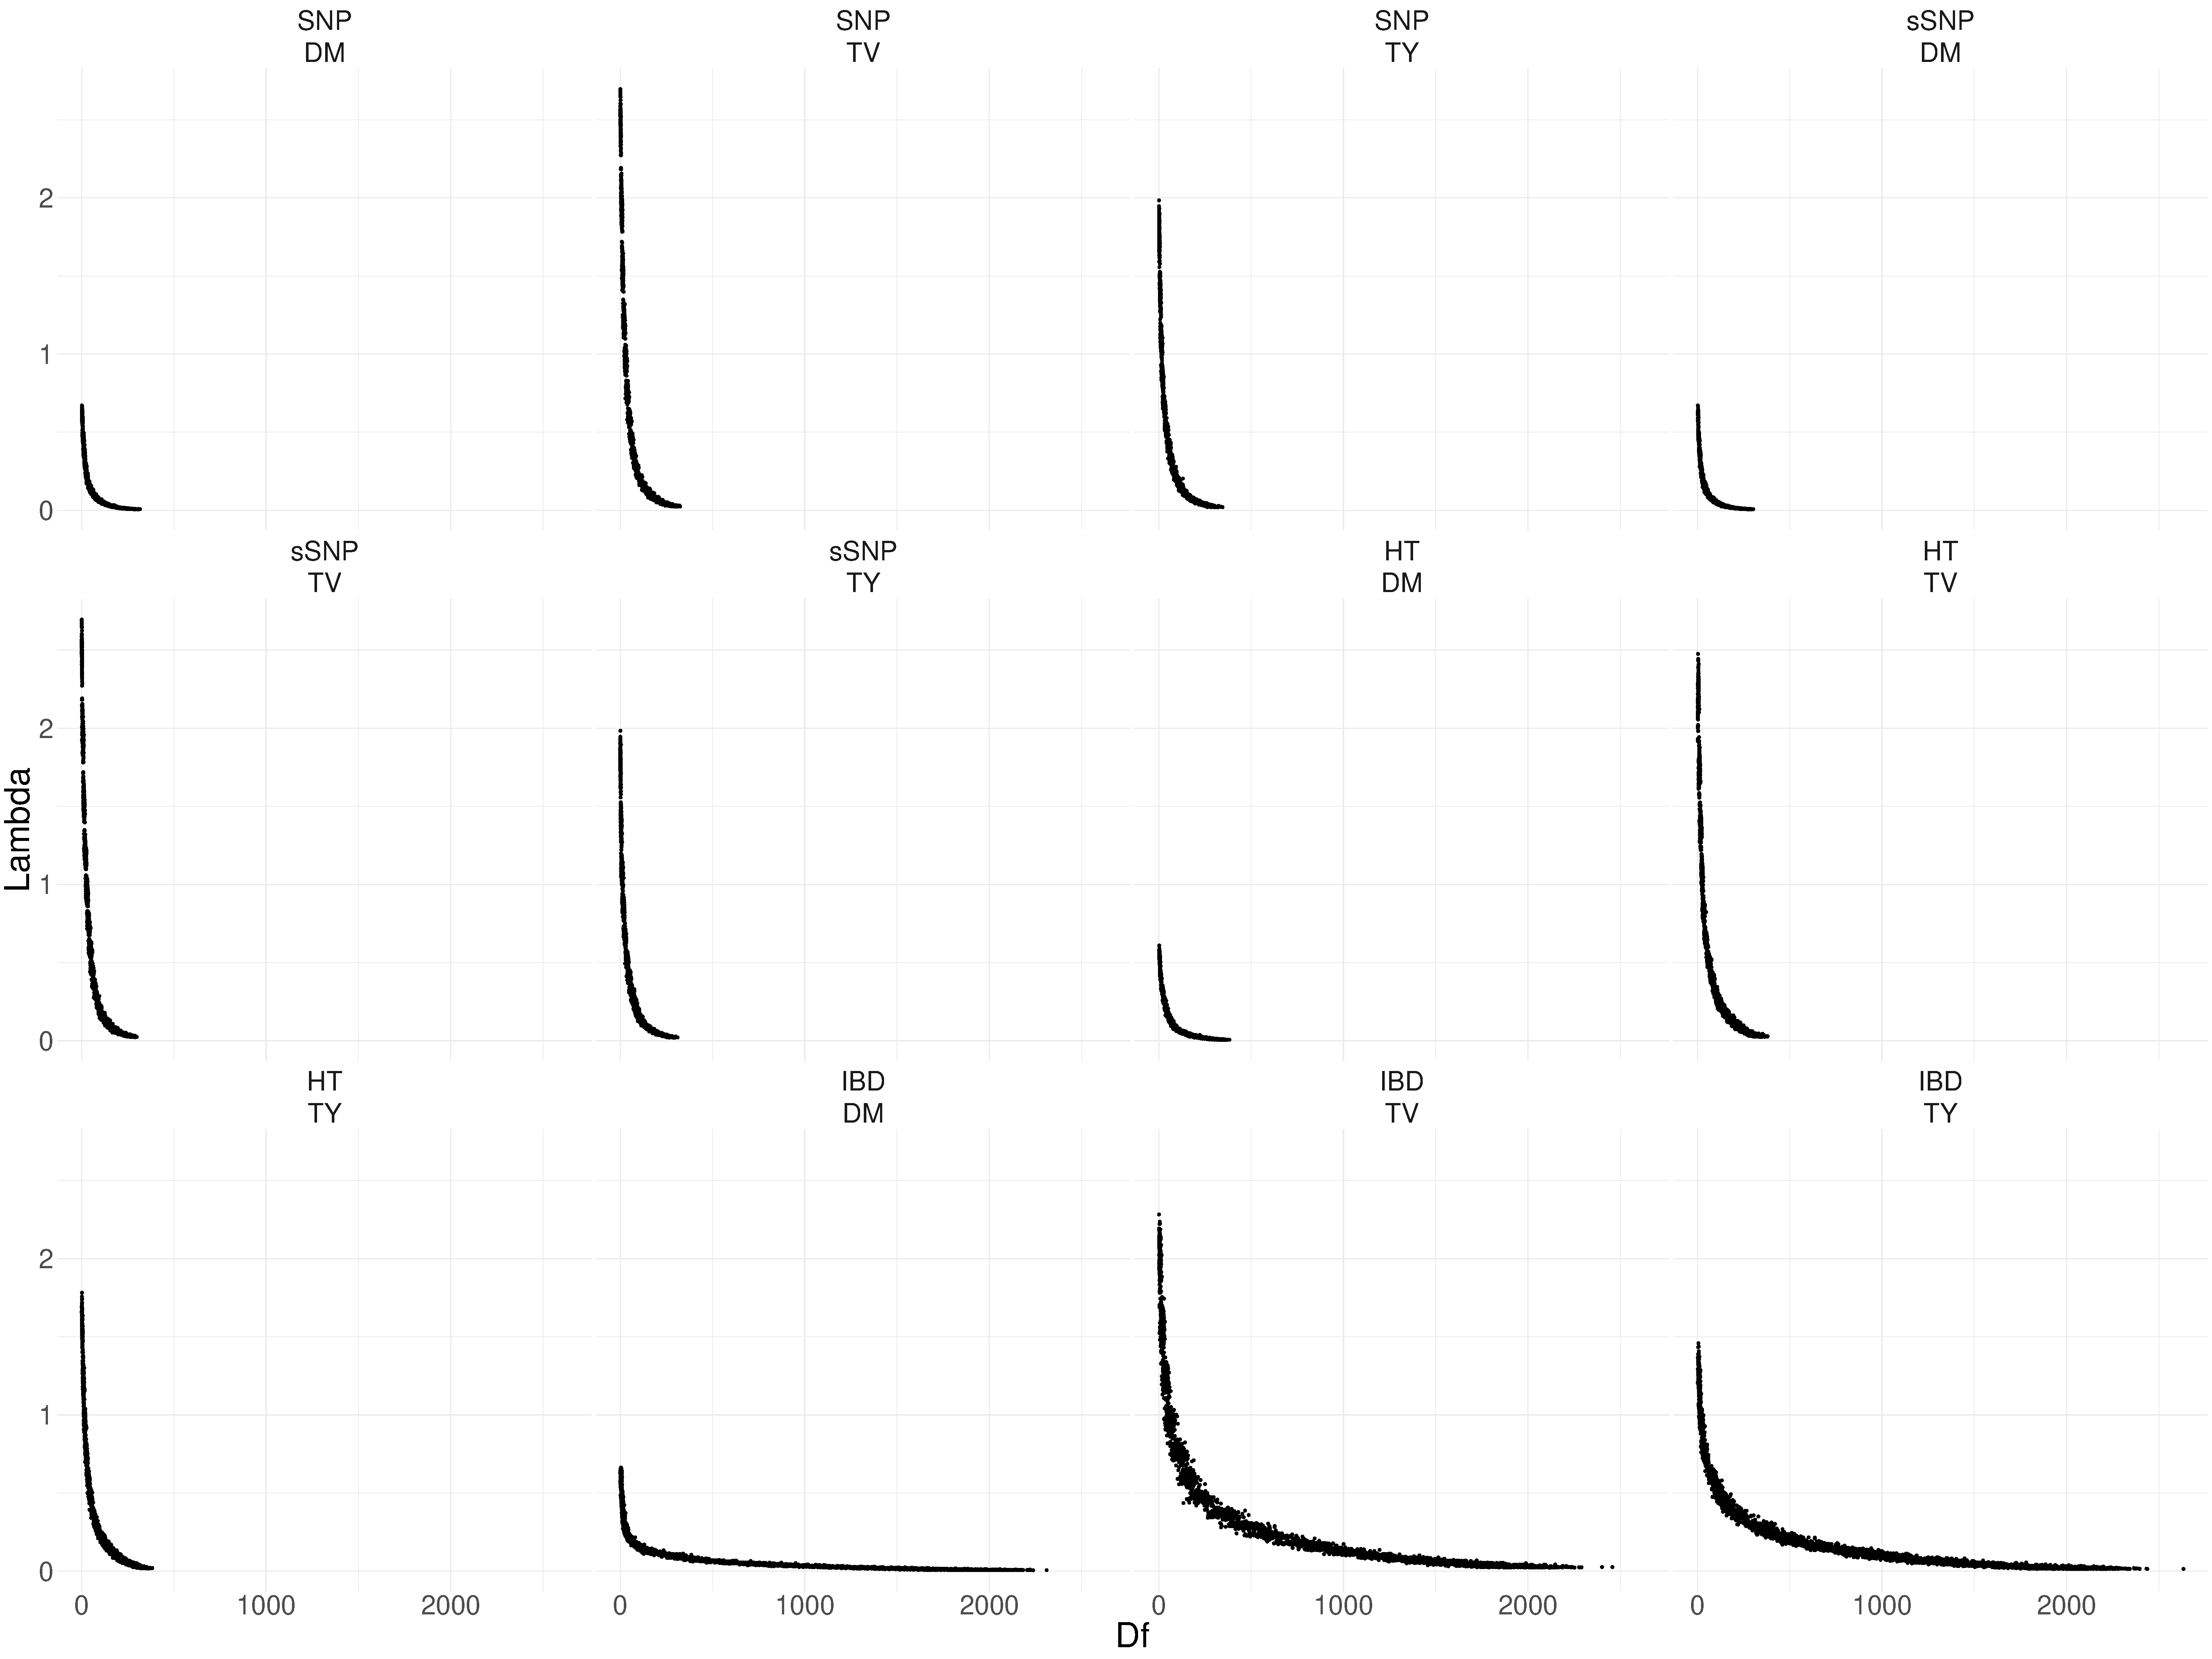
\includegraphics{supplementary_files/figure-pdf/fig-lasso-1.pdf}

}

\caption{\label{fig-lasso}The estimated \(\lambda\) which the associated
degrees of freedom for each predictor set and trait for all lasso
models.}

\end{figure}%

\begin{figure}[h!]

\centering{

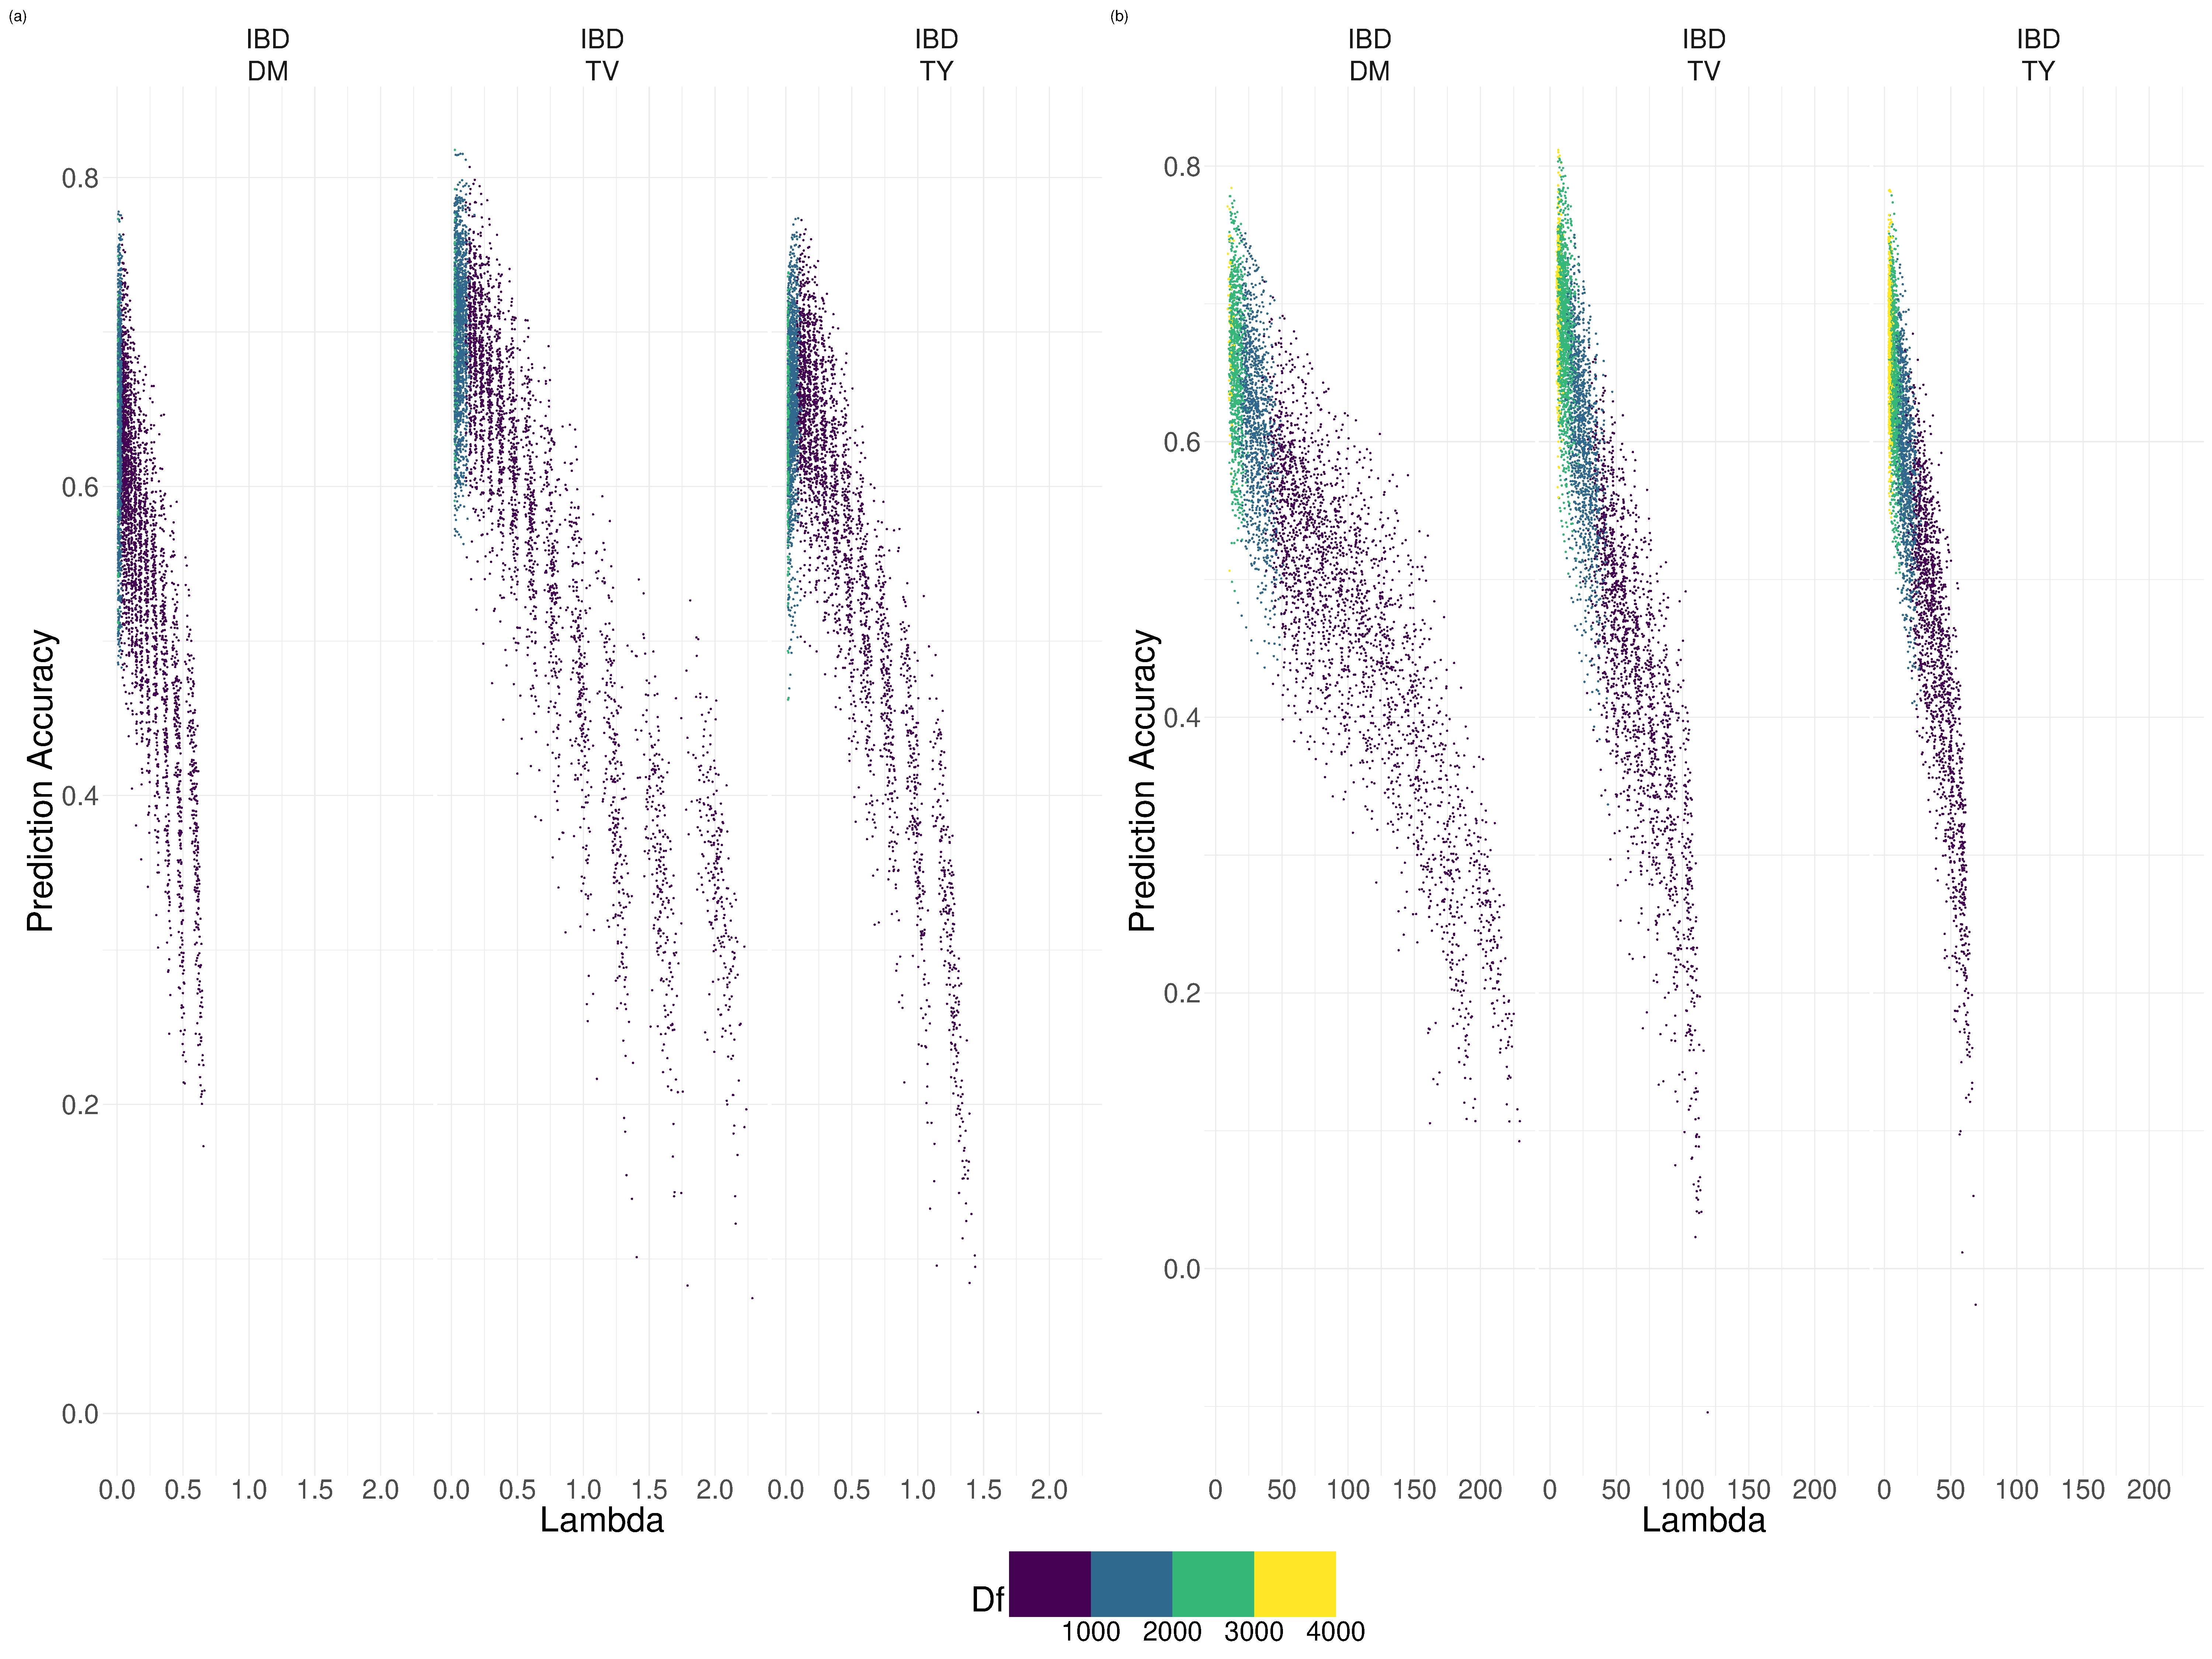
\includegraphics{supplementary_files/figure-pdf/fig-lasso-2-1.pdf}

}

\caption{\label{fig-lasso-2}The estimated \(\lambda\) plotted against
the model prediction accuracy with the associated degrees of freedom for
the multiallelic predictor sets for traditional (a) and (b) grouped
lasso models using IBD-based predictors.}

\end{figure}%

\section{Sampled Posterior Distributions for Gaussian Kernel
parameters}\label{sampled-posterior-distributions-for-gaussian-kernel-parameters}

The Markov Chain Monte Carlo estimation of our parameters for the
Transformed Gaussian Kernel are shown over all runs in (Sup
Fig~\ref{fig-gk-1}) and (Sup Fig~\ref{fig-gk-2}). These represent the
sampled joint posterior distributions of the bandwidth and form
parameters (\((\hat{h},~\hat{\phi})\)) and the estimated genetic and
residual variances
(\((\hat{\sigma}_g\),\textasciitilde{}\(\hat{\sigma}_e)\)),
respectively.

\begin{figure}[h!]

\centering{

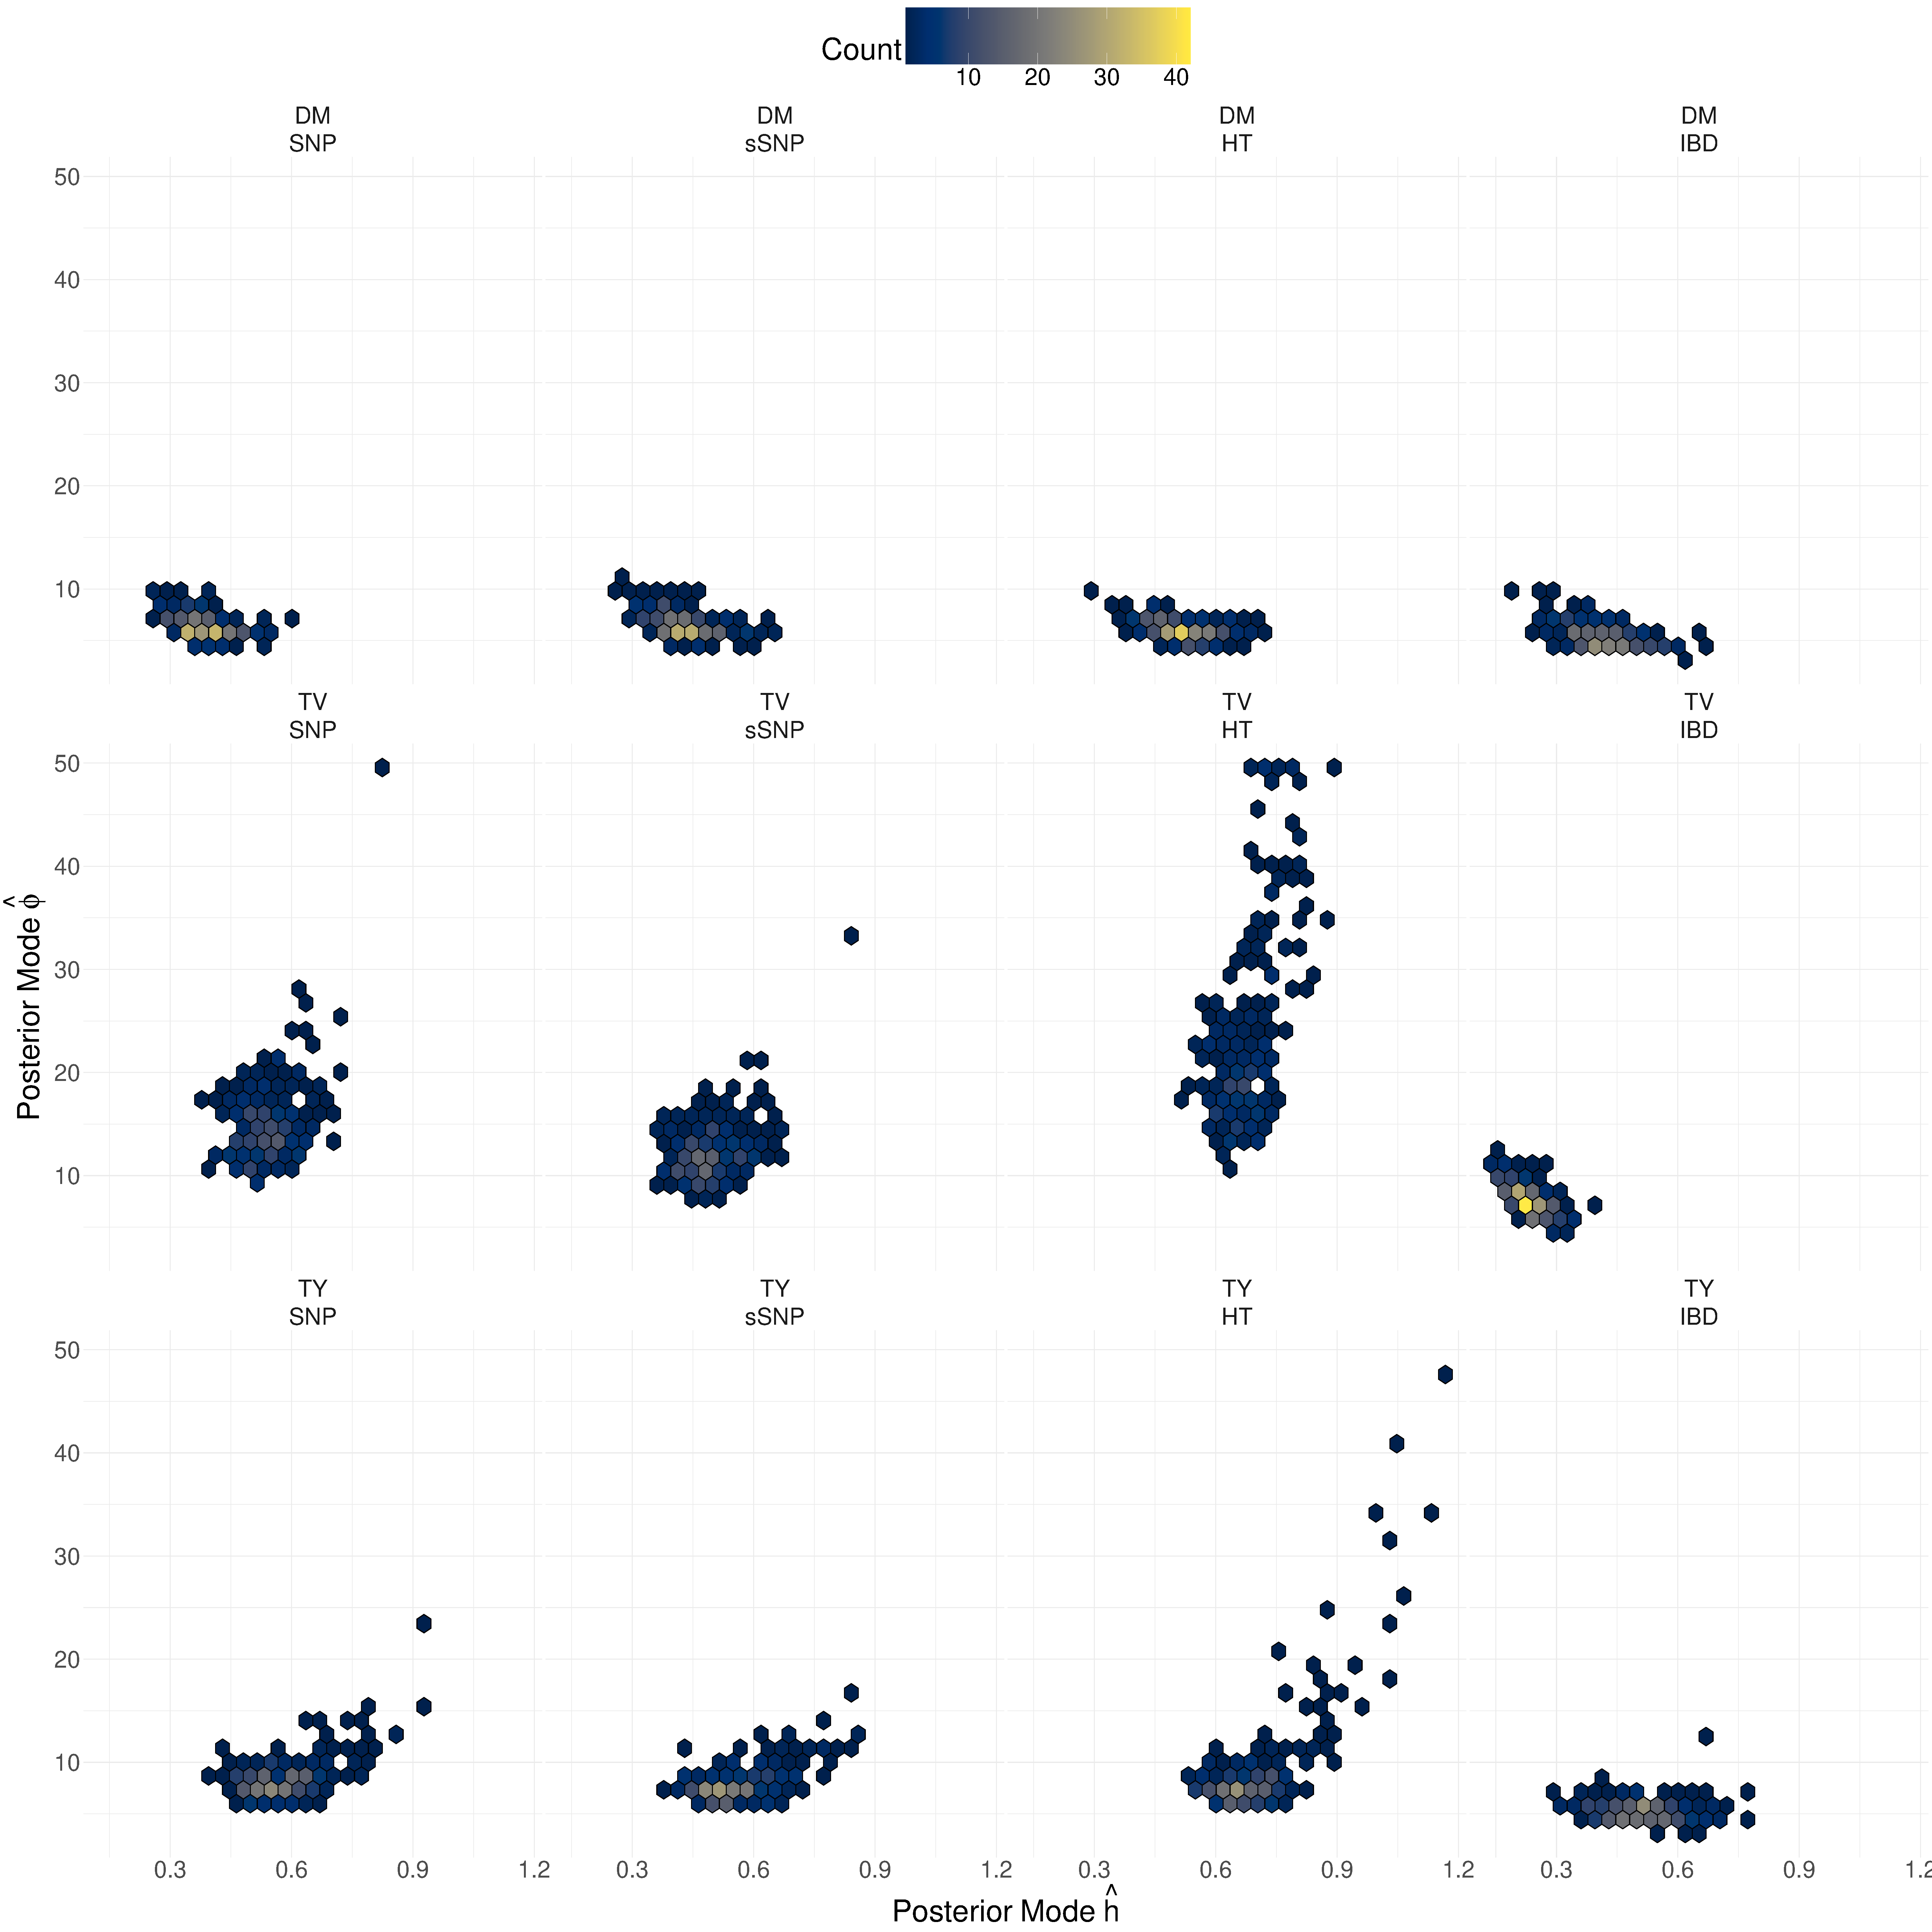
\includegraphics{supplementary_files/figure-pdf/fig-gk-1-1.pdf}

}

\caption{\label{fig-gk-1}Bivariate heat map of the posterior mode of
\(\hat{h}\) and \(\hat{\phi}\) from each fold of the cross-validation
for each trait.}

\end{figure}%

\begin{figure}[h!]

\centering{

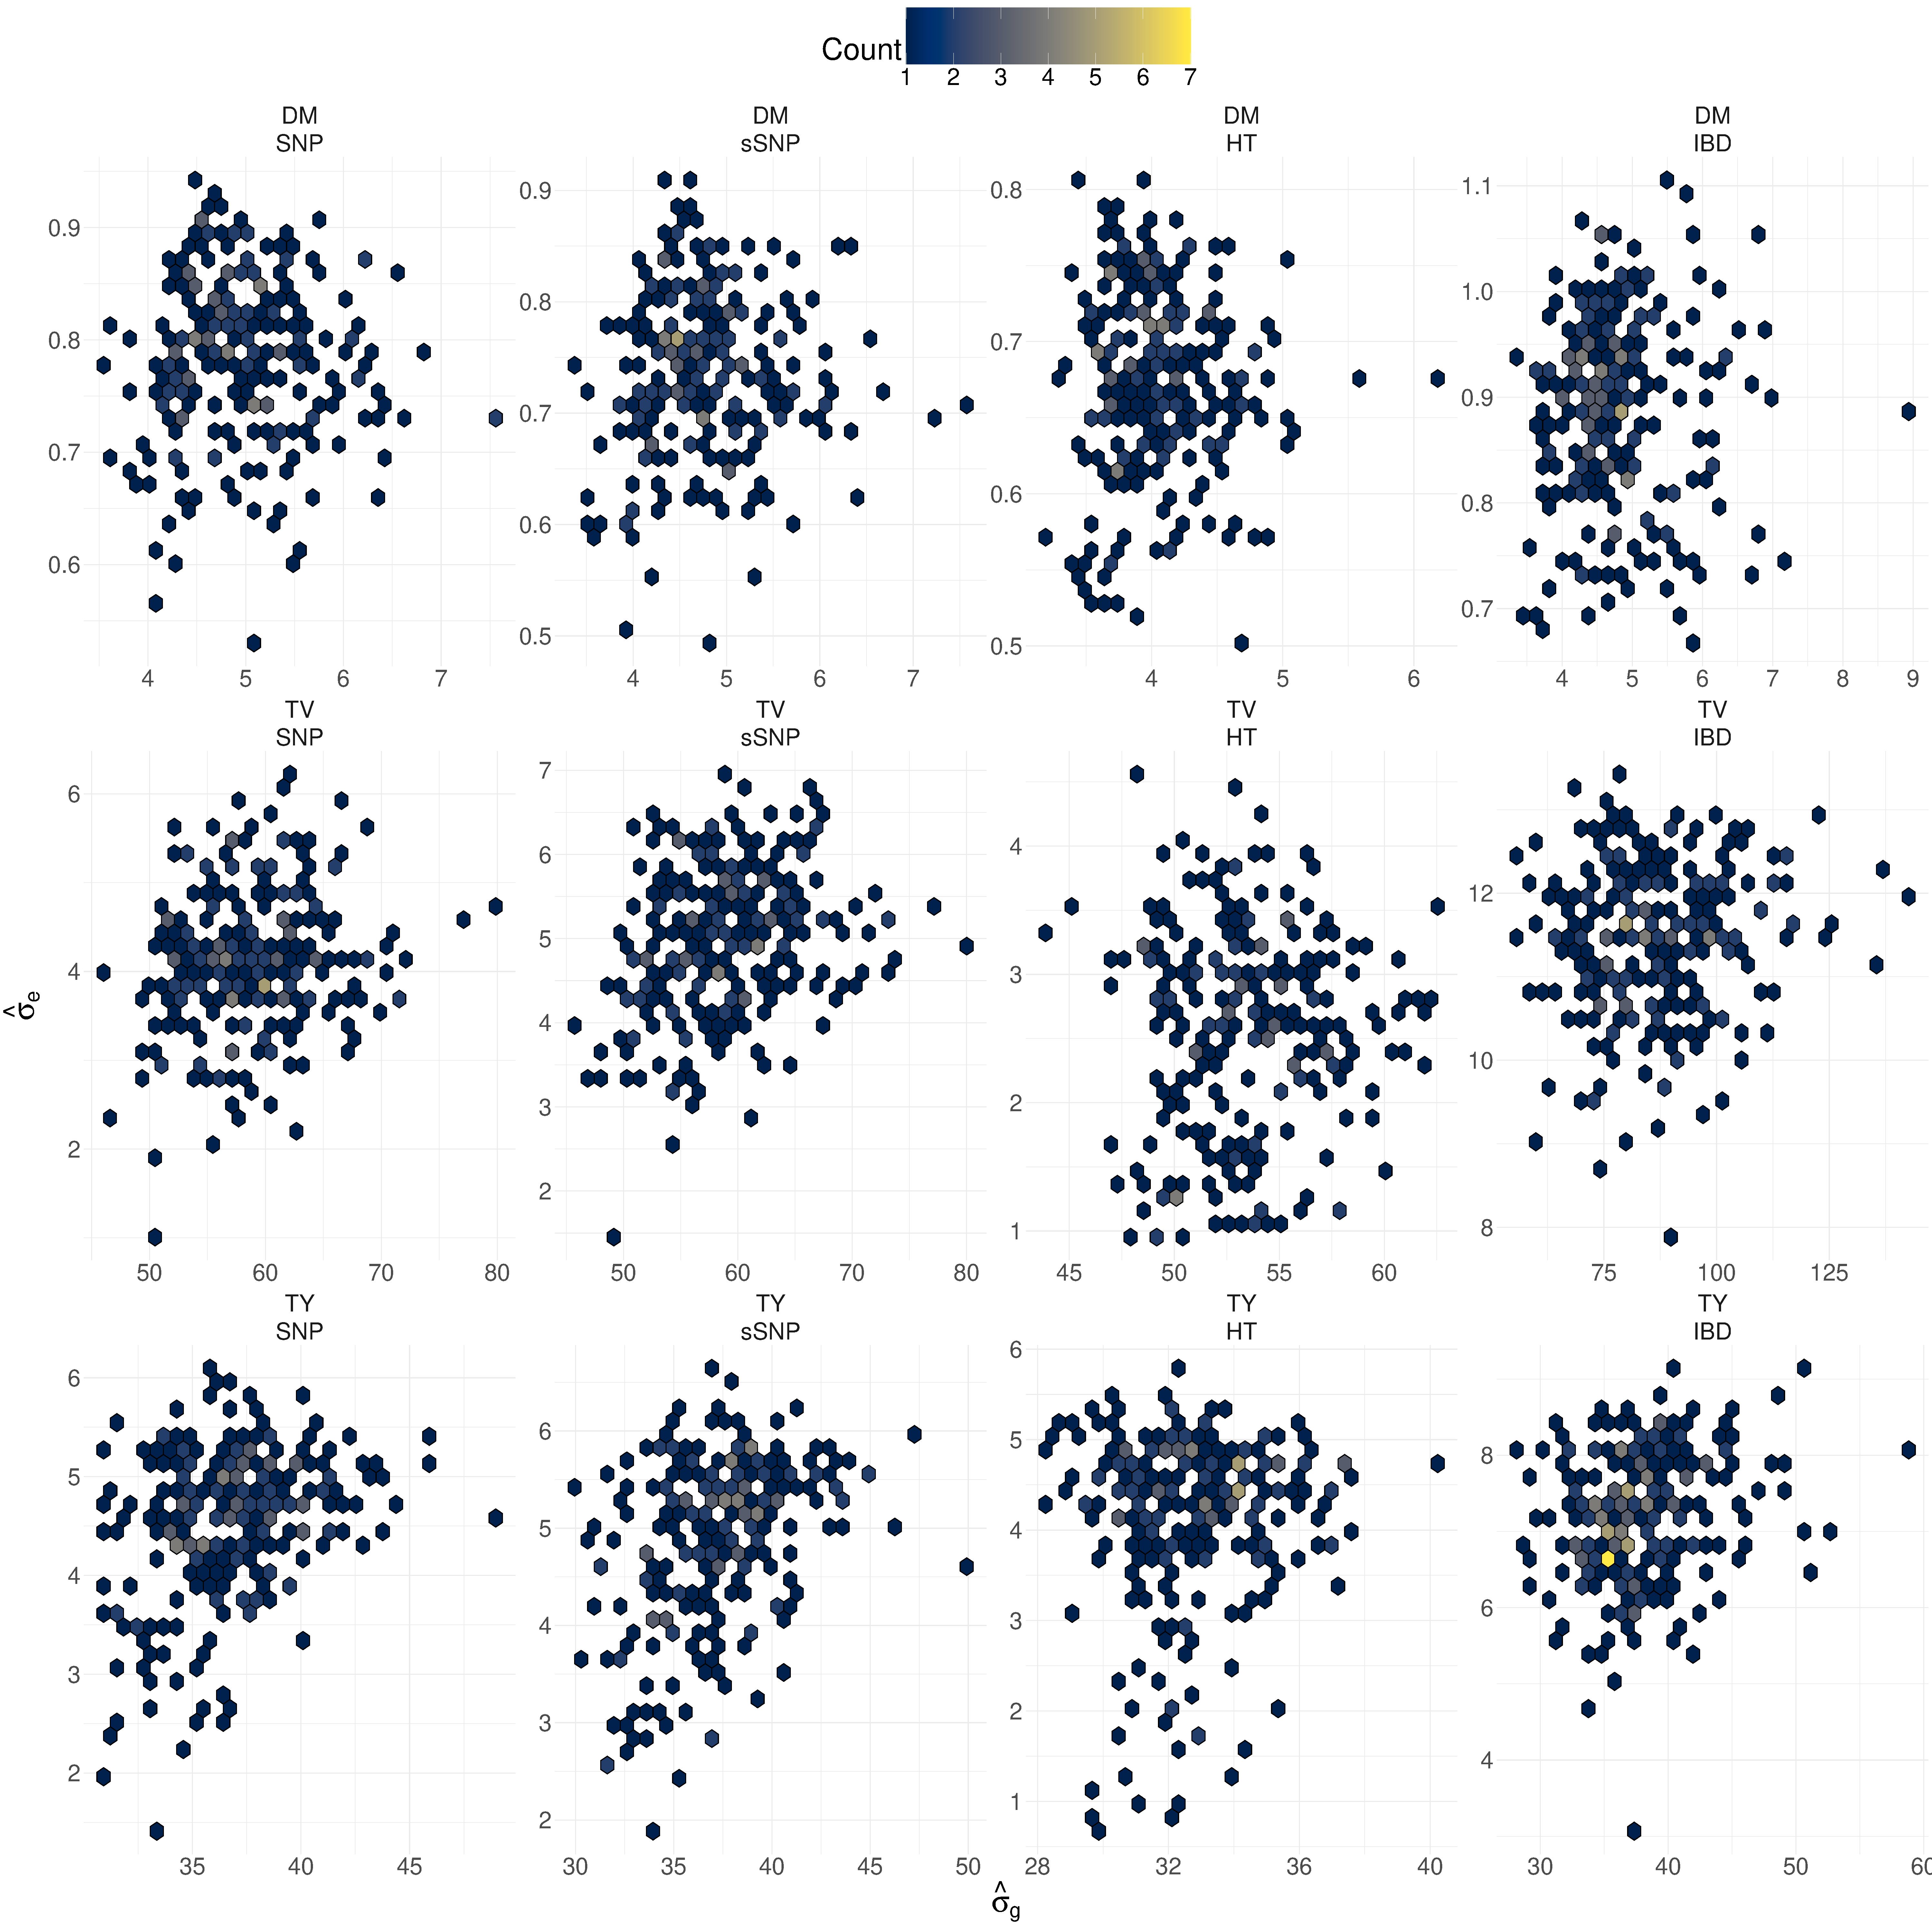
\includegraphics{supplementary_files/figure-pdf/fig-gk-2-1.pdf}

}

\caption{\label{fig-gk-2}Bivariate heat map of the posterior mode of
\(\hat{\sigma_g}\) and \(\hat{\sigma_e}\) from each fold of the
cross-validation for each trait.}

\end{figure}%

